\section{Phase 3: Miniaturisierung und Leistungsanalyse}
\label{subsec:Network_Miniaturization_Performance_Analysis}


\begin{table}[htbp]
\centering
\caption{Konfiguration und Ergebnisse des miniaturisierten Modells}
\label{tab:miniaturization_results}
\begin{tabular}{lc}
\hline
\textbf{Parameter} & \textbf{Wert} \\
\hline
ALPHA & \( 1 \times 10^{-5} \) \\
WORKER & 10 \\
ITERATION & 1 \\
STEPS & 30000 \\
BATCH\_SIZE & 250 \\
EXPLOITATION & 10 \\
LAYERS & 3 \\
LAYER\_1 & 10 \\
LAYER\_2 & 3 \\
NOISE & 0.4 \\
GAMMA & 0.0 \\
\hline
Maximale Belohnung & -4.29 \\
Entsprechende Aktion & [6.84119821, 0.75633377, 0.02226542] \\
\hline
\end{tabular}
\end{table}

Die Ergebnisse der Miniaturisierung sind bemerkenswert, da das verkleinerte Modell eine maximale Belohnung von -4.295256034278478 erreichte, was auf eine nahezu optimale Regelungsleistung hindeutet. Die entsprechenden Aktionen und detaillierten Konfigurationen des Modells sind in Tabelle \ref{tab:miniaturization_results} aufgeführt.

\begin{figure}[htbp]
\centering
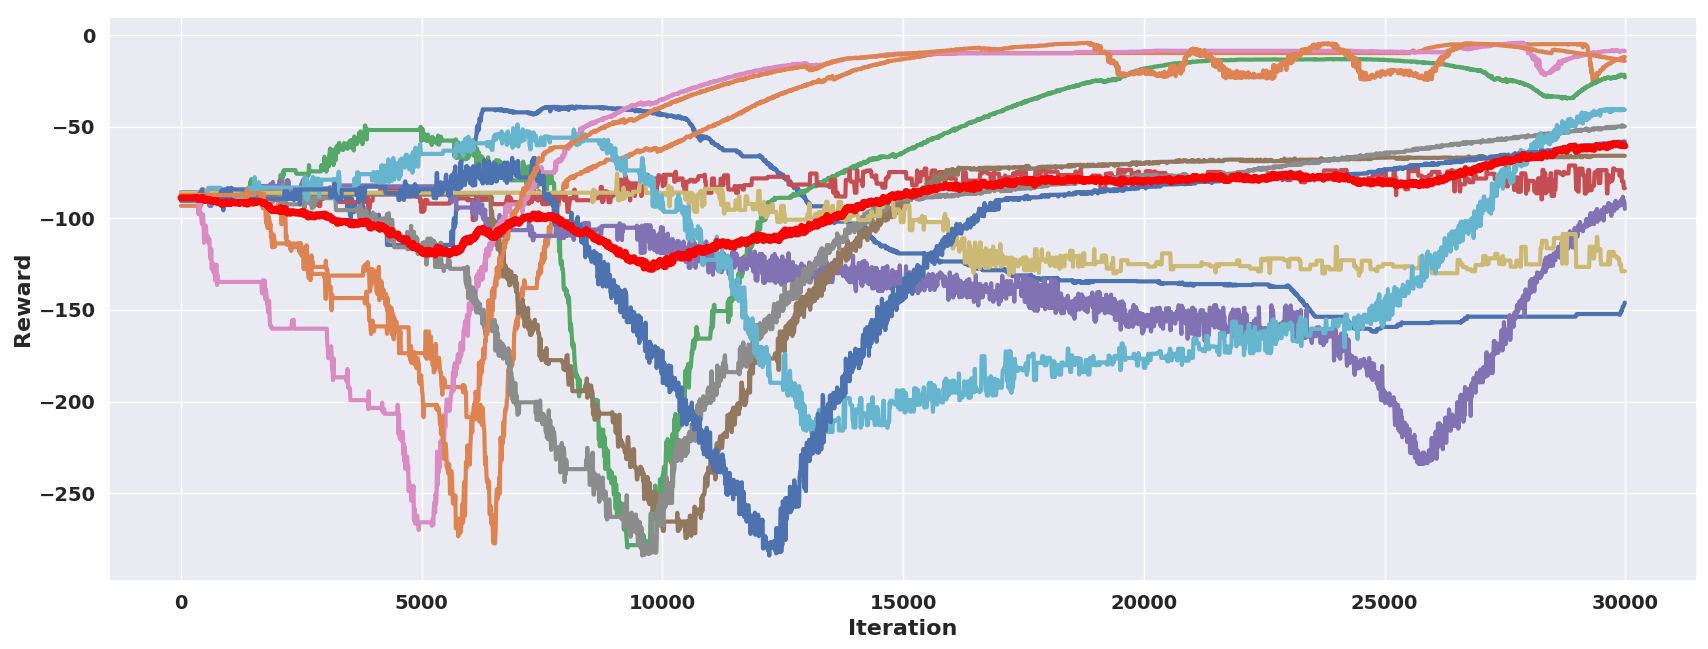
\includegraphics[width=\textwidth]{4Ergebnisse/Phasen/3Phase/3R_big_training_minimize_epoch.png}
\caption{Leistungskurve des miniaturisierten Modells über die Trainingsdauer.}
\label{fig:miniaturized_model_performance}
\end{figure}

Die Leistung des miniaturisierten Modells, wie in Abbildung \ref{fig:miniaturized_model_performance} gezeigt, demonstriert eindrucksvoll, dass eine effiziente Modellminiaturisierung ohne erheblichen Leistungsverlust möglich ist. Diese Erkenntnis ist besonders relevant für praxisnahe Anwendungen, wo kompakte Modelle aufgrund von 
Ressocenbe- schränkungen bevorzugt werden.

Die Ergebnisse wurden durch eine Kombination aus niedriger Lernrate und einer hohen Anzahl von Trainingsepochen erzielt. Die erzielten Ergebnisse \ref{fig:miniaturized_model_performance} weisen darauf hin, dass das Modell trotz der frühzeitigen Beendigung des Trainings bereits eine beachtliche Leistung demonstrierte. Dies legt nahe, dass mit einer Fortsetzung des Trainingsprozesses und einer weiteren Feinabstimmung der Hyperparameter möglicherweise noch höhere Performanzwerte hätten erreicht werden können. Die vorliegenden Ergebnisse bestätigen somit nicht nur die Effektivität des eingesetzten Trainingsansatzes, sondern auch das Potenzial für weitergehende Verbesserungen und Optimierungen.

Ein weiterer wichtiger Aspekt ist das Risiko des Overfittings bei komplexeren Modellen, wie bereits in Kapitel \ref{sec: overfitting} diskutiert. Overfitting tritt auf, wenn ein Modell zu sehr auf die spezifischen Trainingsdaten ausgerichtet ist und dadurch seine Fähigkeit verliert, auf neue, unbekannte Daten angemessen zu reagieren. Es ist eine bekannte Tatsache, dass einfachere Modelle häufig eine bessere Generalisierungsfähigkeit aufweisen, da sie weniger anfällig für das Auswendiglernen spezifischer Trainingsdaten sind. Unsere Ergebnisse zeigen, dass das miniaturisierte Modell trotz seiner Einfachheit eine gute Leistung erbringen konnte, was die Wichtigkeit einer ausgewogenen Modellkomplexität in der Modellentwicklung hervorhebt. 

Insgesamt legen diese Beobachtungen nahe, dass es vorteilhaft sein kann, sich auf die Optimierung von Hyperparametern zu konzentrieren, um kleinere, aber leistungsfähige Modelle zu entwickeln.
